The wage gap is an oft-cited number that quantifies the difference between males and females in the economy: In the fourth quarter of 2016, white women earned 81.1\% as much as white men and African American women earned 92.1\% as much as African American men. This reveals a gap not only by gender, but also by race with African American women (men) only earning 67.8\% (73.6\%) as much as white men.\footnote{\citet{USDPTL_2017_Wage_News-Release}.}

 Although this favors males, there are related measures of gender differences that favor females. In 2015, only 64 (103) per 100,000 (African American) females were incarcerated in comparison to 488 (2,613) per 100,000 (African American) males.\footnote{\citet{UDOJ_2016_PrisonersStatistics_Bulletin}.} Similarly, in 2012-2013, more females than males received bachelor's degrees across all races with large disparities for African Americans: 65\% of degrees conferred to African Americans were conferred to females.\footnote{\citet{UDOE_2016_Statistics_Report}.}

These differences are select measurements from the life-cycle trajectory of skill formation and labor market opportunities. Based on previous literature of skill formation, these later skills build on earlier skill development.\footnote{\citet{Cunha_Heckman_2008_JHR,Cunha_Heckman_etal_2010_est_tech_cognoncog}.} Additionally, higher levels of these skills, especially social-emotional skills, can lead to more positive life-relevant outcomes like health.\footnote{\citet{Heckman_2008_EI,Heckman_Pinto_etal_2013_PerryFactor,Conti_etal_2016_LongTermHealth}.} The adult gender differences highlighted above can be the result of early differences that propagate over the life-cycle. Policy interventions can widen or close the gaps between males and females. We examine these differences by analyzing the effects of two nearly identical early childhood interventions. 

The interventions, the Carolina Abecedarian Project (ABC) and the Carolina Approach to Responsive Education (CARE), were randomized controlled trials using a sample of disadvantaged families in Chapel Hill, North Carolina with children born between 1972 and 1980. We combine the samples of the two interventions and denote this combined sample ABC/CARE. The children in the treatment group attended high-quality, intensive, early childhood education from birth until age 5. The families in the control group were not granted access to this center-based treatment, and instead either kept their children in informal care with relatives or enrolled them in alternate center-based care. Researchers collected measures of cognitive, social-emotional, and parenting skills on the subjects in both the treatment and control groups during and after the intervention. Data follow-ups are available into adulthood and cover a wide variety of important domains, such as education, employment, and health.

To connect the ABC/CARE sample with the gender differences listed above, we present select gender differences of skill measurements in Figure~\ref{fig:intro-skills-plots-skills}.\footnote{More gender differences are presented in Appendix~\ref{}.} Females perform, on average, about five quantiles better than males on early measures of social-emotional skills.\footnote{This is consistent with previous work showing that females tend to outperform males on tests of skills \citep{Baker-Milligan_2013_Boy-Girl-Differences}.} There is a similar gender difference in the early measures of parenting, specifically the absence of punishment. That is, in the ABC/CARE sample, males receive more parental discipline than their female counterparts. Stark gender differences are not present in IQ or achievement measures. 

We can also examine the gender differences in adult outcomes (Figure~\ref{fig:intro-skills-plots-adultsimp}). The gender differences for income and education are not significantly different, however, males have slightly higher levels of both. Health, represented by adult BMI, is worse for females by about five quantiles. This difference is reversed when considering costs from criminal activity, which is consistent with the national gender differences.\footnote{These crime costs are estimated in \citet{Garcia_etal_2016_Comp_CBA_Unpublished}.} 

\begin{figure}[!htbp]
\centering
\caption{Differences Between ABC/CARE Males and Females}
\label{fig:intro-gdiff-plots}
\begin{subfigure}[h]{0.55\textwidth}
	\centering
	\caption{Skill Measurements}
	\label{fig:intro-skills-plots-skills}
	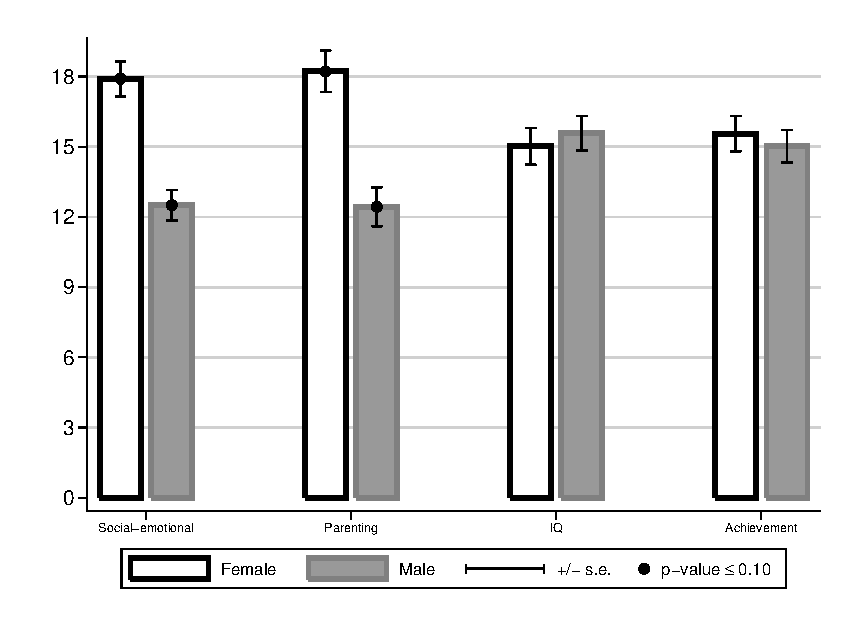
\includegraphics[width=\textwidth]{../output/abccare-gdiff-skills}
\end{subfigure}

\begin{subfigure}[h]{0.55\textwidth}
	\centering
	\caption{Adult Outcomes}
	\label{fig:intro-skills-plots-adultsimp}
	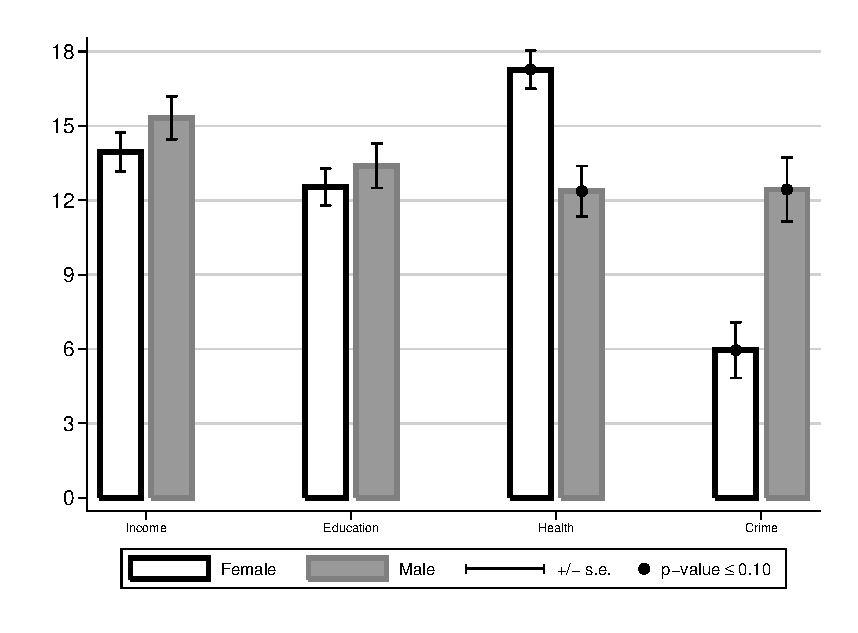
\includegraphics[width=\textwidth]{../output/abccare-gdiff-adultsimp}
\end{subfigure}
\footnotesize \justify
Note: These plots show the means of select variables by gender, pooling across experimental groups. The capped lines show the standard errors and black points indicate that the female is significantly different than the males. These hypothesis tests are two-sided and computed using 100 bootstraps. All factor variables are calculated by principal factor analysis. The factors are then standardized and divided into 30 quantiles. Panel (a) Social-emotional is a factor of task-orientation measured by the Infant Behavioral Record (IBR; \citet{Bayley_1969_BSID-Manual}) at ages 0.5, 1, 1.5 years. Parenting is a factor of the absence of punishment scale of Home Observation for Measurement of the Environment (HOME; \citet{Elardo_Bradley_1981_DR}) between ages 0.5 and 4.5 years. IQ is a factor of full IQ scores measured by the Stanford-Binet Intelligence Scale (SB; \citet{Terman_Merrill_1960_BOOKSBintelligence}), McCarthy Scales of Children's Abilities (MC; \citet{McCarthy_1972_Manual-McCarthy-Scales}), and the Wechsler Preschool and Primary Scale of Intelligence (WPPSI; \citet{Wechsler_1974_Manual-WISC-R}) at ages 2, 3, 4, and 5 years. Achievement is a factor of reading and math scores measured by between the ages of 6 and 12 years. Panel (b) Income is the lifetime net present value of income predicted in \citet{Garcia_etal_2016_Comp_CBA_Unpublished}. Education is an indicator of high school graduation by 21 years. Heath is BMI measured at approximately 35 years. Crime is the net present value of projected crime costs as estimated in \citet{Garcia_etal_2016_Comp_CBA_Unpublished}. All of these adult variables are standardized and split into quantiles to be consistent with the skills.
\end{figure}

Although these mean differences do not include the effect of early childhood education on improving these skills, many studies have shown the potential for early-life interventions to improve the skills of children, especially those from disadvantaged families.\footnote{\citet{Currie_2011_AER,Elango_Hojman_etal_2016_Early-Edu}.} Several of these studies separate analysis by gender and find that males and females benefit differently from early childhood education. For example, \citet{Heckman_Moon_etal_2010_QE} and \citet{Garcia_etal_2016_Comp_CBA_Unpublished}, both of which analyze randomized control trials with long-term data follow-ups, find that intervening early in life more positively affects education for females and labor market and health outcomes for males. Other studies analyzing programs with shorter-term data also find gender differences in early skills and academic outcomes.\footnote{\citet{Deming_2009_AEJAE,Ou_Reynolds_2010_Mechanisms_CYSR,Magnuson_Kelchen_Duncan_etal_2016_ECRQ}.} 

This paper studies the treatment effects of ABC/CARE by gender to clearly present the relationship between gender differences and early childhood education's effect on those differences. We compute standard treatment effects comparing the treatment and control group. This considers the treatment effect given that the control-group families select the ``next best'' early childhood option for their children. This option can include staying at home or attending other center-based care.\footnote{Historical documentation, records, and evidence from knowledgeable individuals indicate that although these alternate centers followed state and federal standards, they were of lower quality than the ABC/CARE intervention.} Unlike previous studies analyzing ABC/CARE, we additionally compute treatment effects comparing the treatment group to the control group fixing those in the control group to these alternate counterfactuals.\footnote{Previous studies presenting treatment effects of ABC and CARE include \citet{Ramey_etal_1985_Project-CARE_TiECSE, Clarke_Campbell_1998_ABC_Comparison_ECRQ,Campbell_Pungello_etal_2001_DP,Campbell_Ramey_etal_2002_ADS,Campbell_Wasik_etal_2008_ECRQ,Campbell_Conti_etal_2014_EarlyChildhoodInvestments}.}$^,$\footnote{See \cite{Heckman_1992_randomization}, \cite{Heckman_Hohmann_etal_2000_QJE}, and \cite{Kline_Walters_2016_QJE} for work related to control substitution.} 

Given the large number of available variables from the numerous follow-ups, summarizing across these treatment effects can be reductive.\footnote{We consider 95 outcomes that are able to be monetized.} \citet{Garcia_etal_2016_Comp_CBA_Unpublished} offer one solution by presenting a benefit/cost analysis. This analysis aggregates across the outcomes that can be monetized and weights those effects by the social cost. This exercise indicates that the benefits from ABC/CARE are largely driven by the effects on males: The benefit/cost ratio is 10.19 for males and 2.61 for females. We present a complementary method to aggregate treatment effects without weighting by social cost. This aggregate, a combining function, counts the number of positive (and significant) treatment effects by gender. In contrast to the benefit/cost ratio, this aggregate indicates that females benefit more from the program than do males. This seemingly contradictory result is explained by the types of treatment effects by gender and specific gender differences. For example, although the treatment reduced crime for both males and females, males tend to commit more costly crimes (e.g. violent crimes that have large costs to the victim). We explain the treatment effects in detail to help explain the gender differences present in these aggregate estimates.

We find strong effects on education and employment for females with high school graduation increasing between 13 and 25 percent and employment increasing between 8 and 13 percentage points.\footnote{The range arrises from the different estimates.} Although the treatment did not increase education for males as strongly as for females, it increased employment between 11 to 19 percentage points and labor income between 19 and 24 thousand of 2014 US dollars.\footnote{Income, employment, and education were measured when the subjects were 30 years.} 

We broaden the discussion of results to the full set of outcomes by presenting the estimates of the counts of positive treatment effects. To perform inference on these estimates, we test the hypothesis of whether the proportions are equal to 50\%. As Figure~\ref{fig:intro-cfunctions} shows, although the proportions for both genders are significantly greater than 50\%, the proportion is higher for females. When considering the proportion of outcomes that are both positive and significant at the 10\% level, we test the hypothesis whether the proportions are equal to 10\%. A similar pattern holds for this test as well, although the proportions are smaller. Across outcomes, the effects are stronger for males fixing the control group to alternate preschool, but stronger for females when fixing the control group to staying at home. This pattern holds in the individual treatment effects, the combining functions, and the results from \citet{Garcia_etal_2016_Comp_CBA_Unpublished}.

\begin{figure}[!htbp]
\centering
\caption{Proportion of Outcomes that are Positively Impacted}
\label{fig:intro-cfunctions}
	\begin{subfigure}[h]{0.7\textwidth}
		\centering
		\caption{Treatment vs. Next Best} \label{fig:ppositivenb}
		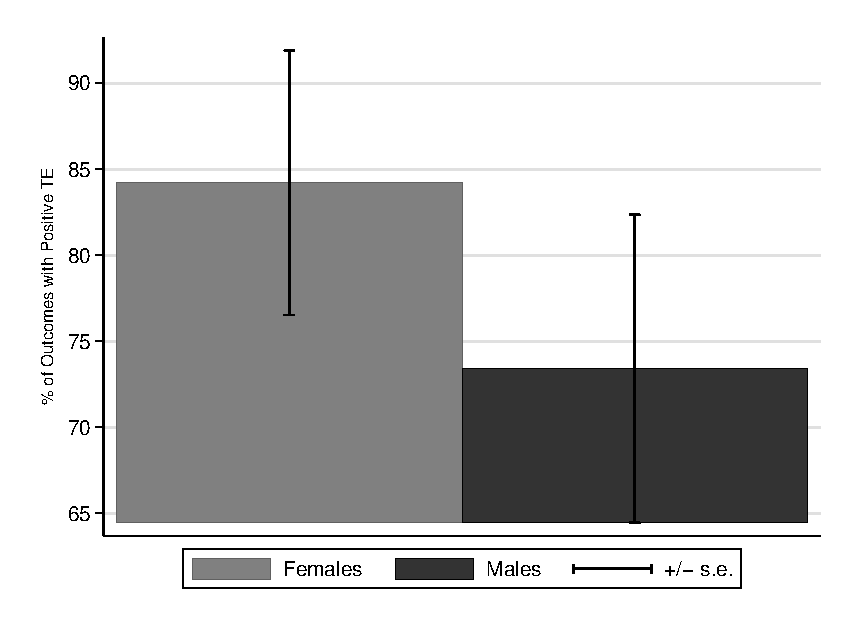
\includegraphics[width=\textwidth]{../output/itt_noctrl_all.eps}
\end{subfigure}

\begin{subfigure}[h]{0.7\textwidth}
	\centering
	\caption{Treatment vs. Next Best, Significant at 10\% Level} \label{fig:ppositive10}
		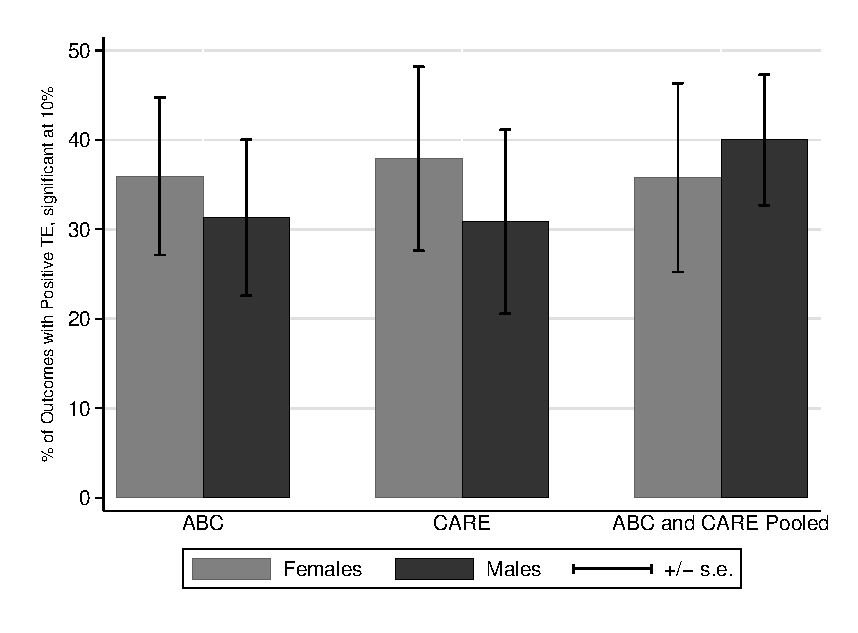
\includegraphics[width=\textwidth]{../output/itt_noctrl_all_sig10.eps}
\end{subfigure}
\footnotesize \justify
Note: Panel (a) percentage of outcomes displaying a positive treatment effect, comparing treatment to next best. Panel (b) percentage of outcomes displaying a positive and statistically significant treatment effect (10\% significance level). 
\end{figure}

This difference in the results depending on the counterfactual, as well as the gender differences in the treatment effects, drives our discussion of the interaction between the treatment, the family inputs, and any potential alternate center-based care. The explanation that males are more fragile than females early in life is consistent with the early differences favoring females.\footnote{\citet{Kottelenberg-Lehrer_2014_Gender-Effects,Baker_Gruber_Milligan_2015_Noncog_Defects, Schore_2017_IMHJ}.} Building on this, we explore how these early-life differences evolve for specific outcomes that are central to the analysis of  \citet{Garcia_etal_2016_Comp_CBA_Unpublished}, such as crime and income.

The paper proceeds as follows. We describe ABC/CARE in more detail in Section~\ref{sec:data}. We then discuss the parameters of interest in Section~\ref{sec:parameters} and describe our method for summarizing over the multitude of variables in Section~\ref{sec:combining-functions}. Section~\ref{sec:treatment-effects} displays the estimates of the parameters of interest and the combining functions. We discuss suggestive mechanisms through which the early-life skill differences mediate later-life gender differences in Section~\ref{sec:gender-differences}. Section~\ref{sec:conclusion} concludes.

%ee \citet{Beeghly-etal_2017_IMHJ,Dayton_2017_IMHJ,Iruka_2017_IMHJ,Schore_2017_IMHJ} for recent findings on the topic of different development of males and females early in life. 